\begin{center}
{\Large {\bf Figures}}
\vspace{1.5cm}
\end{center}
%
%\begin{figure}[h!]
%\begin{center}
%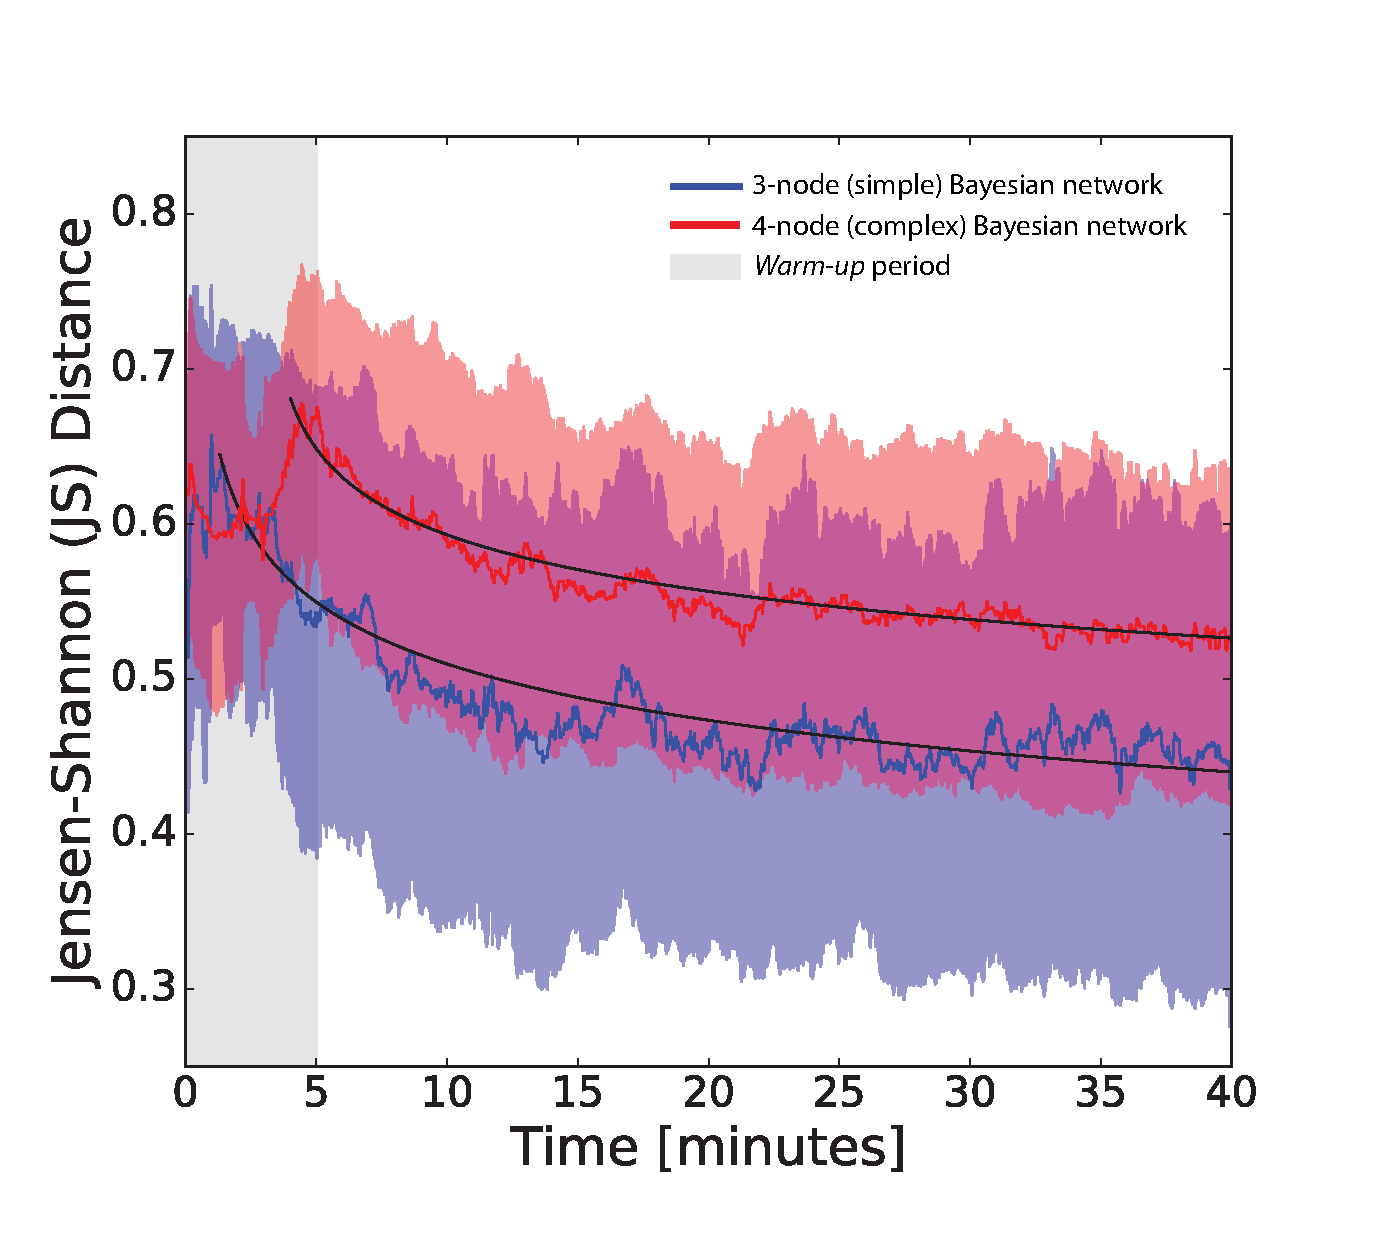
\includegraphics[width=12cm]{figures/decay_simple_complex.eps}
%\caption{\footnotesize Decay of the Jensen-Shannon (JS) Distance (\ref{JS-distance}) between models proposed by participants and the true model over time for the 3-node (simple) and 4-node (complex) Bayesian network treatments (resp. in blue and red). The colored areas show the standard deviation. The decays are averaged (mean) over all participants for each treatment. Both treatments follow similar extremely slow power law decay (\ref{power_law_decay}), yet with different exponents: $\alpha = 0.1$ ($p < 0.001$, $R = -0.92$) for the simple Bayesian network treatment and $\alpha = 0.07$ ($p < 0.001$, $R = -0.94$) for the complex Bayesian treatment. The grey area on the left shows the 5-minute {\it warm up} period during which participants get used to the interface. In both treatments, participants elaborate initial Bayesian Net models with $JSD \approx 0.6$, and there is a phase associated with counter-performance (during which the JS Distance increases). This phase is however much shorter for the simple Bayes Net (peak at $t \approx1$ minute) compared to the complex Bayes Net (peak at $t \approx 4.5$ minutes) after which the JS-distance actually starts to decay.}
%\label{fig:decay}
%\end{center}
%\end{figure}

%\begin{figure}[h!]
%\begin{center}
%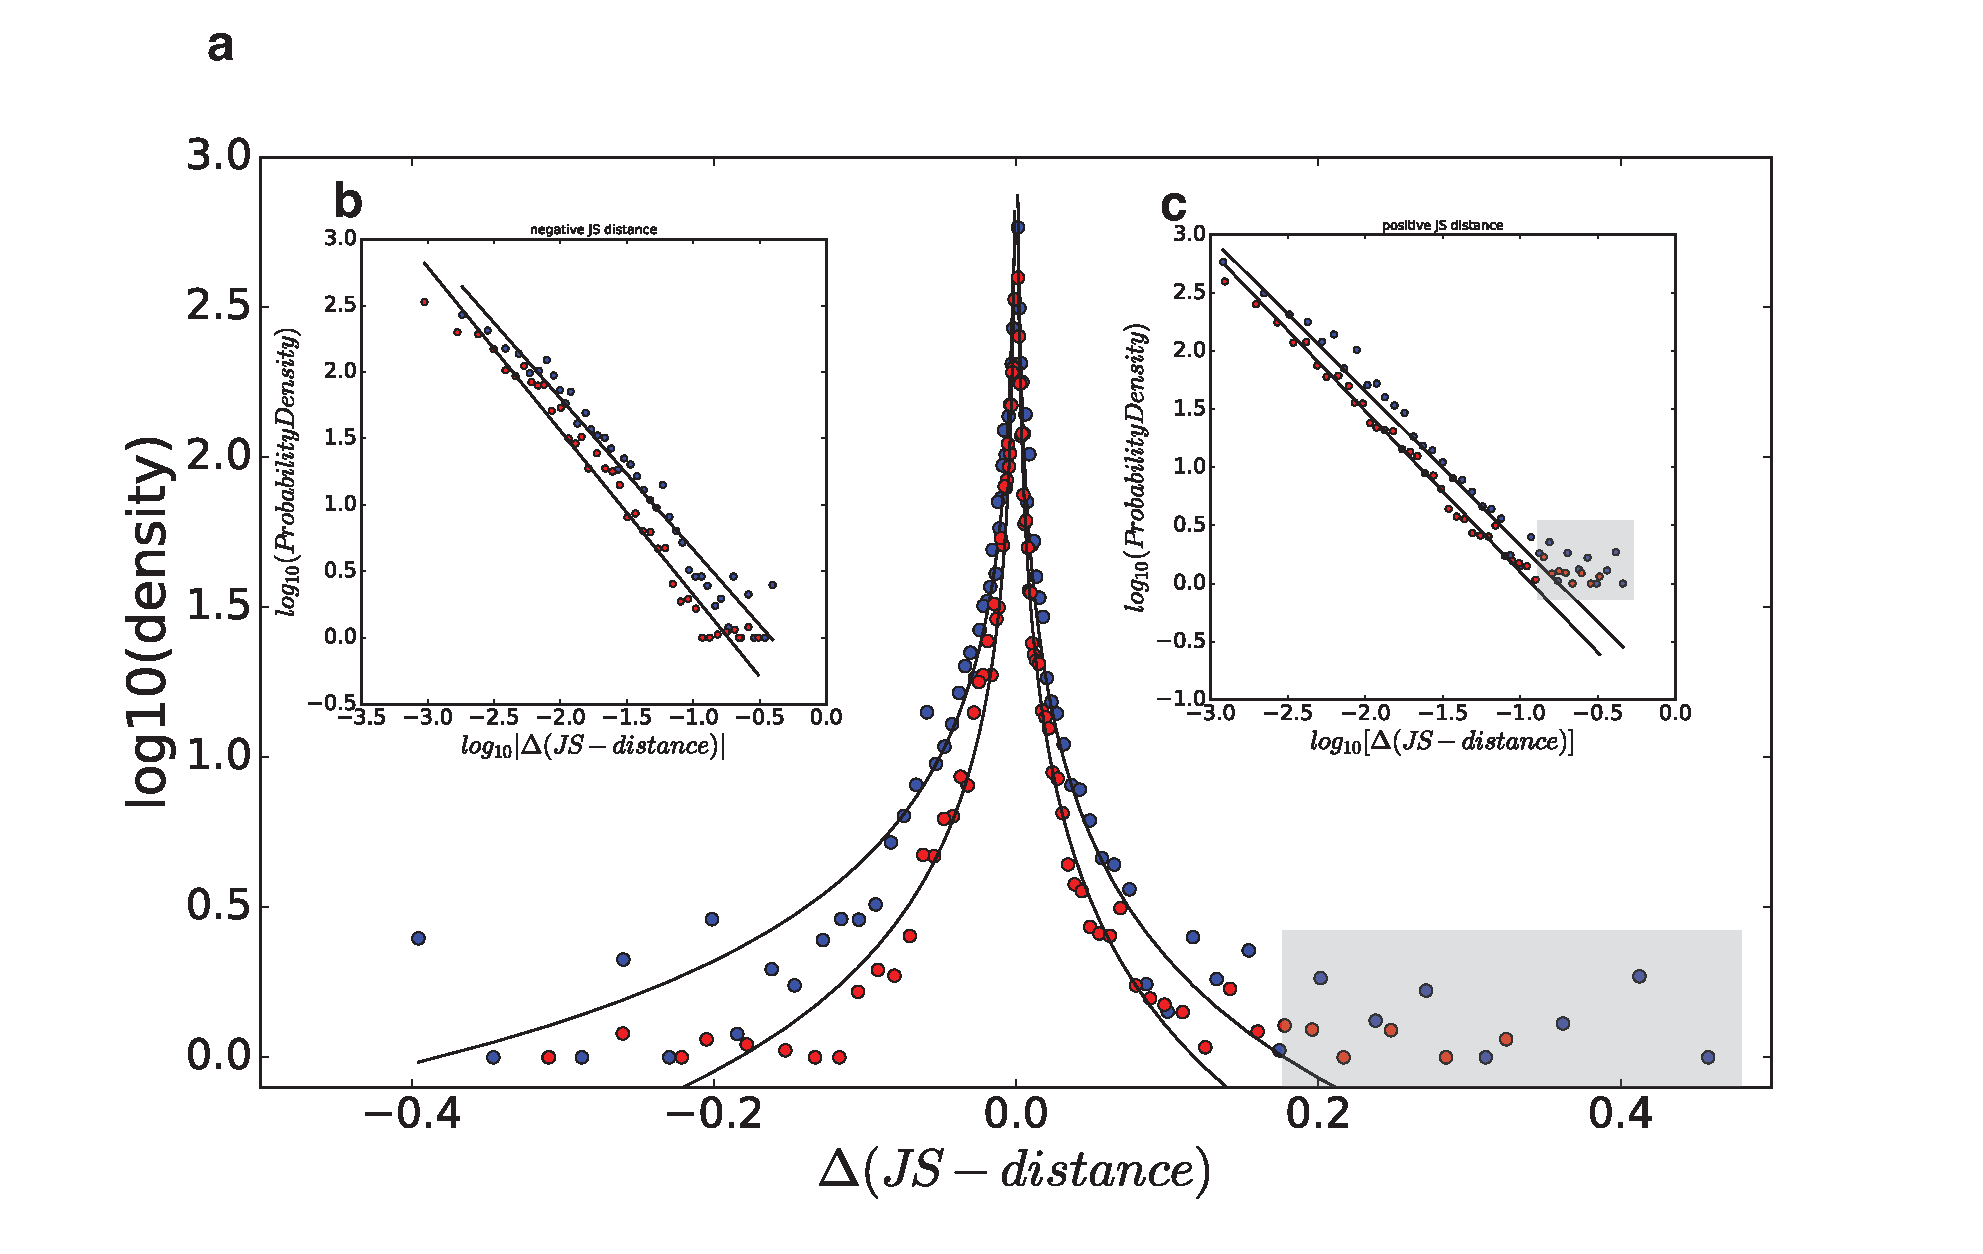
\includegraphics[width=15cm]{figures/pdf_JSD.eps}
%\caption{{\bf a.} Probability density function (un-normalized) of $\Delta(JS-distance)$ ($\Delta JSD$) between 2 consecutive changes (jump sizes). The negative $\Delta(JS-distance) < 0$ stands for improvement (i.e., the goal is to reduce the $JS-distance$). On the contrary, the $\Delta(JS-distance) >  0$ happens when a participant comes up with a BayesNet model which is further from the true model, compared to the previous attempt. The distribution is heavy-tailed on both sides (c.f., {\bf b.} and {\bf c.}), almost power law tail, yet with some particularities: For $\Delta JSD < 0$, the probability density function may be a {\bf log-normal}. For $\Delta JSD > 0$, an extra ``outliers" regime is present (grey shade rectangle). Also, $\Delta JSD > 0$ is more heavy-tailed compared to $\Delta JSD < 0$ (see Table \ref{pwlaw_fits}). The {\it simple} and {\it complex} treatments (resp. blue and red dots) look similar, yet with sligtly different exponents (see again Table \ref{pwlaw_fits}). Interestingly, the median in both simple and complex cases is very close to zero [$median(pdf) < 0.001$], which means that on average, after a change was made to a model the model is only a slight improvement over the old.}
%\label{fig:jump_sizes}
%\end{center}
%\end{figure}

\begin{figure}[h!]
\begin{center}
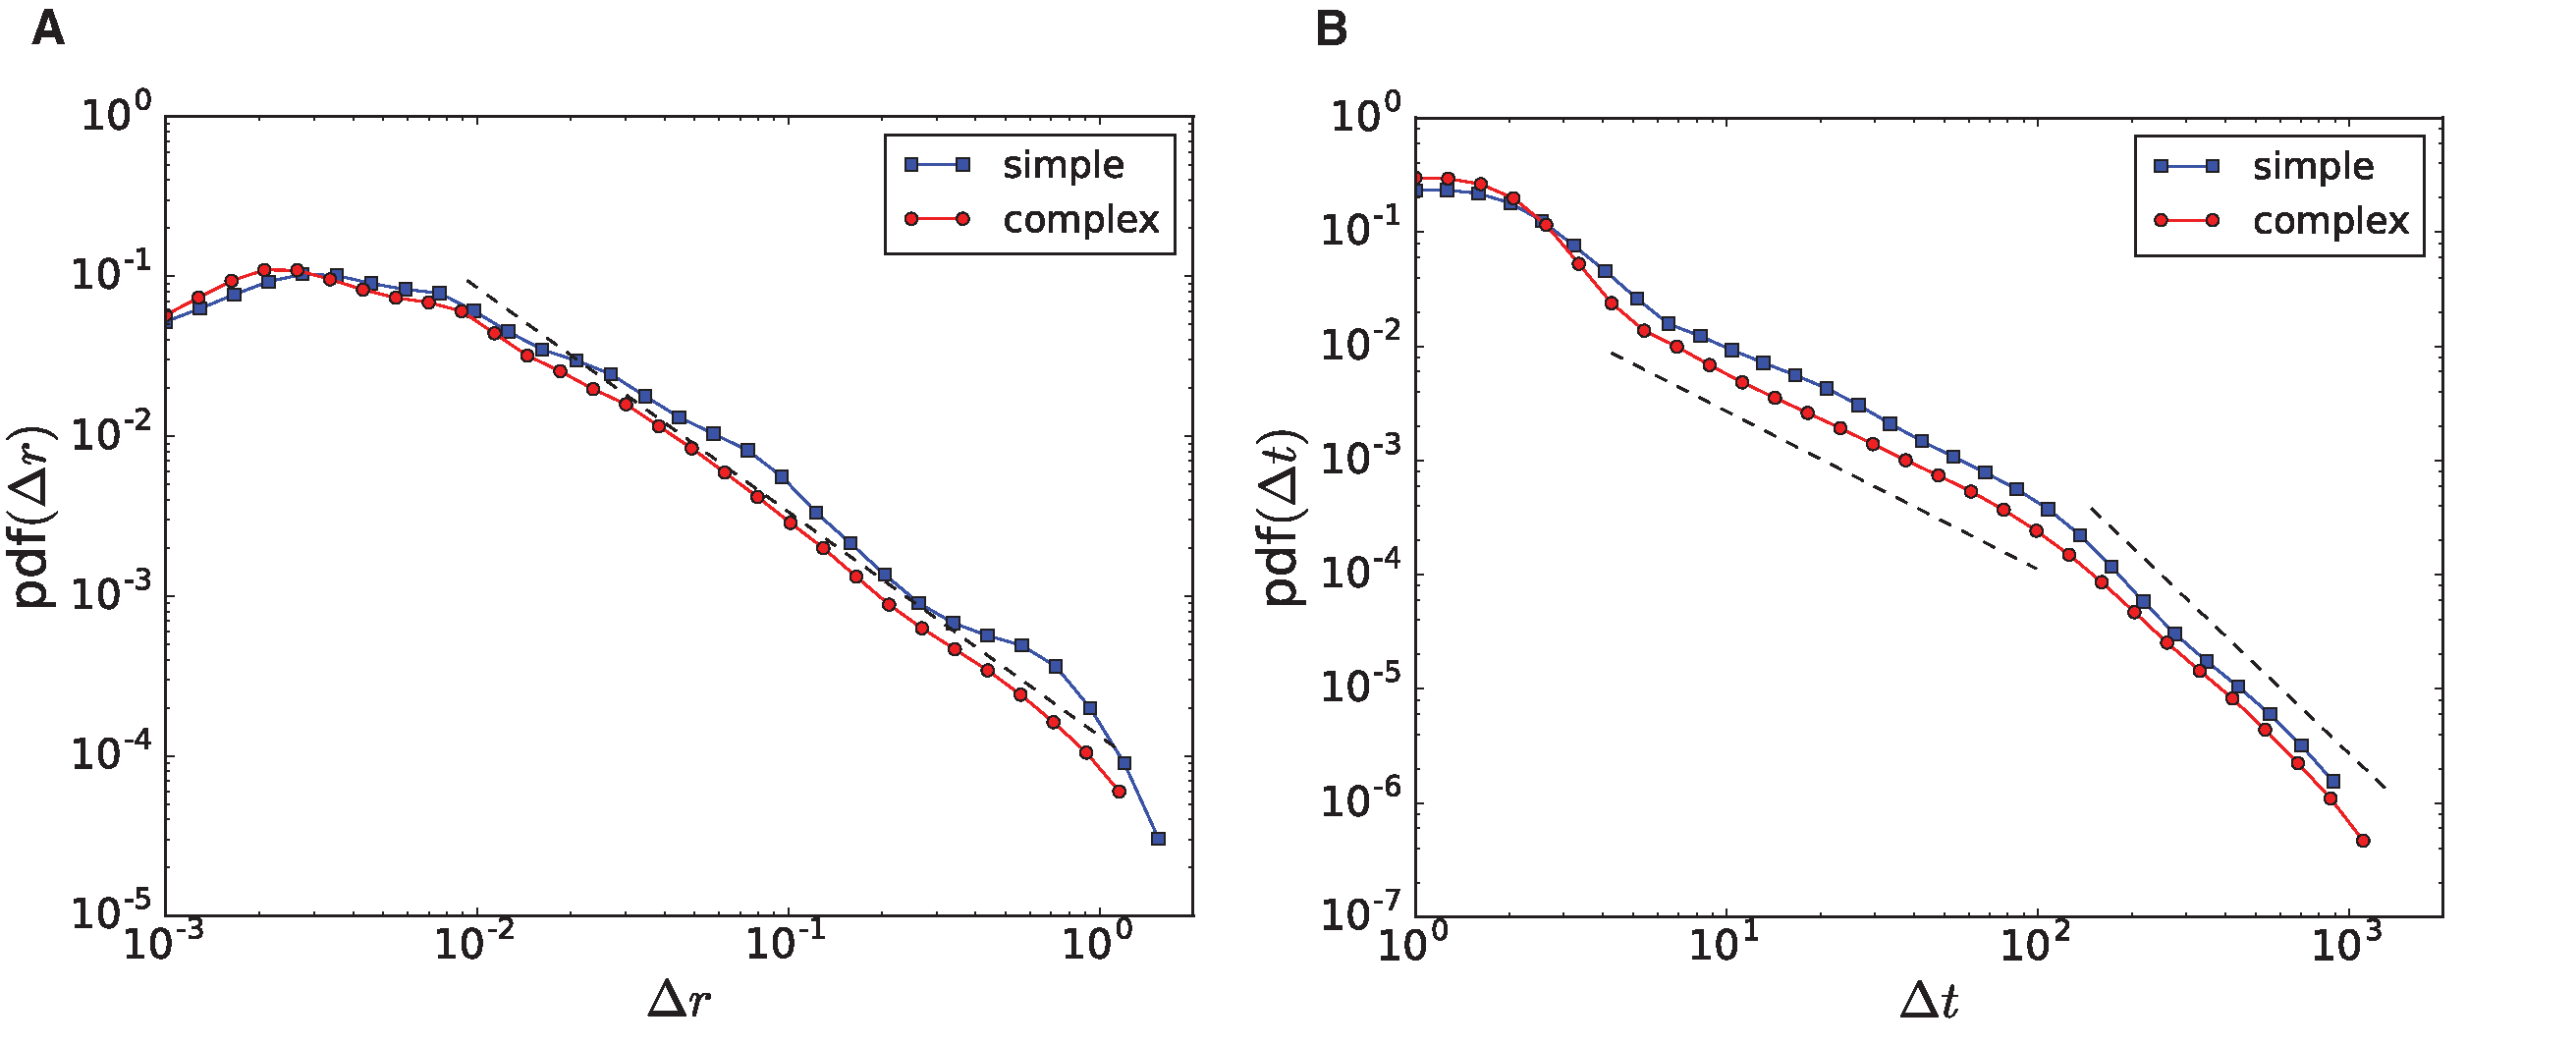
\includegraphics[width=17cm]{figures/pdfs.pdf}
\caption{{\bf A.} Probability density function of displacement $pdf(\Delta r) = \Delta r^{-\alpha -1}$ with $\alpha = 0.40(5)$. {\bf B.} Probability density function of waiting time $\Delta t$ $pdf(\Delta t) = \Delta t^{-\beta -1}$ with 2 regimes : $\beta_{\Delta t < 125} = 0.38(4)$ and $\beta_{\Delta t > 125} = 1.59(5)$. Distributions of $\Delta r$ and $\Delta t$ are equivalent for the simple and complex treatments.}
\label{fig:pdfs}
\end{center}
\end{figure}




%\begin{figure}[h!]
%\begin{center}
%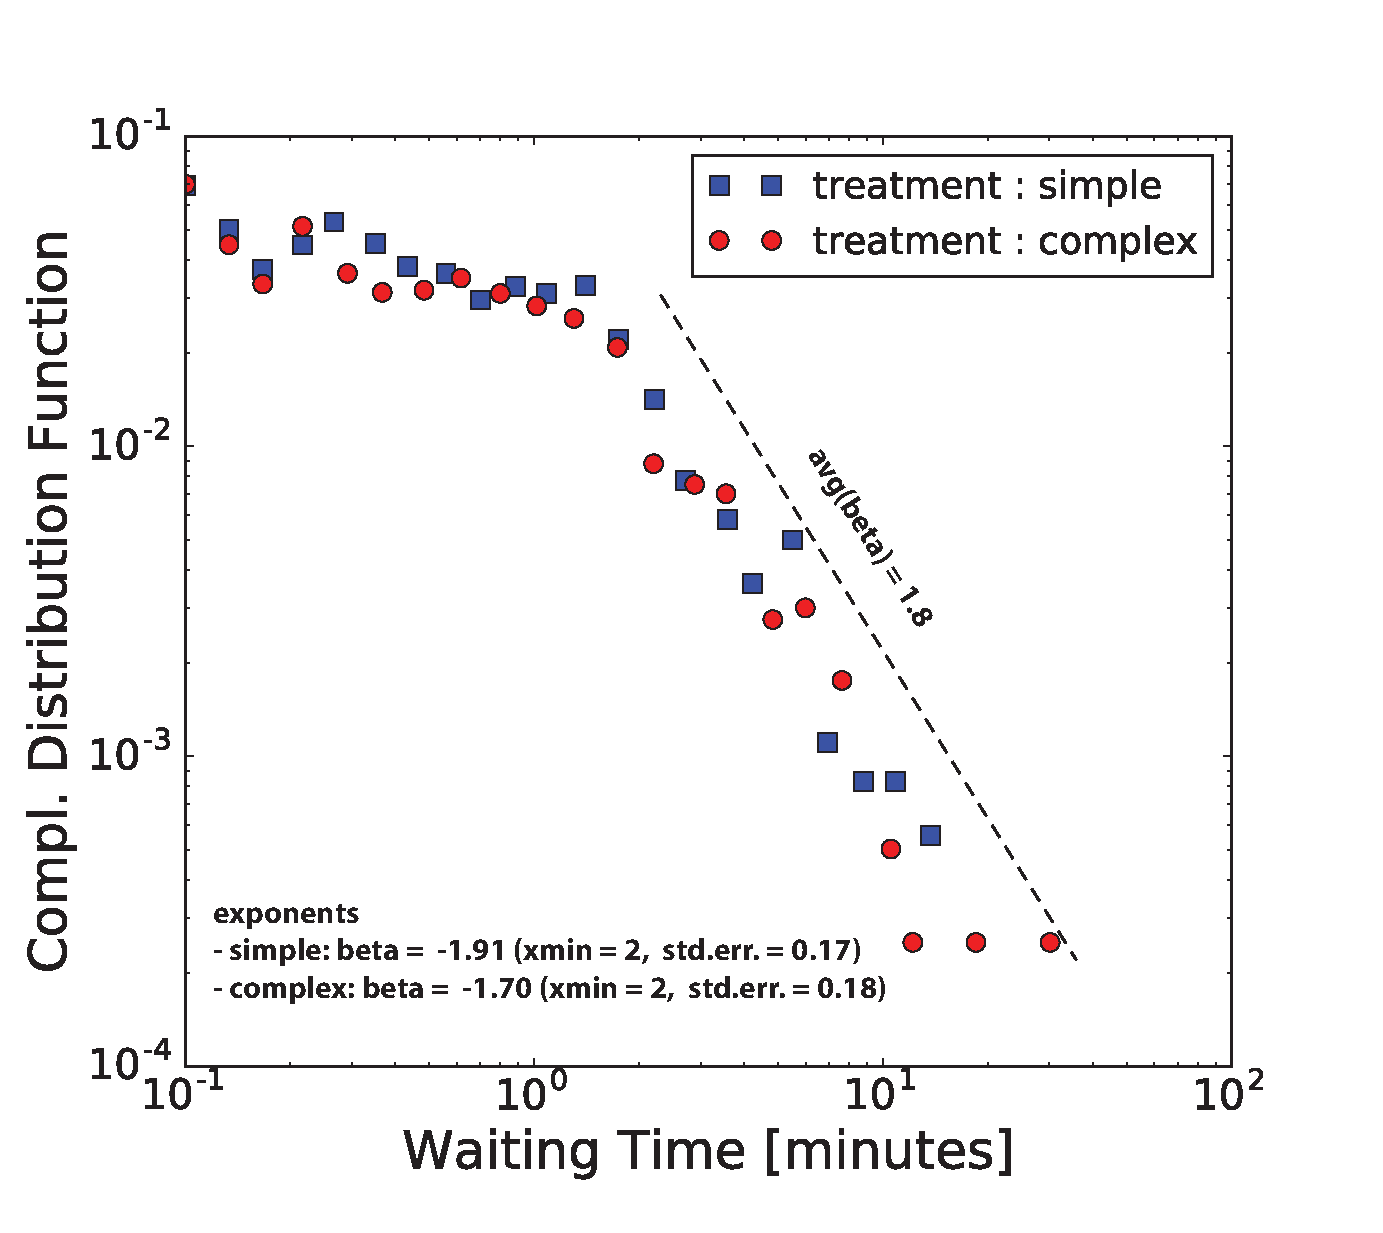
\includegraphics[width=15cm]{figures/ccdf_waiting_time.eps}
%\caption{Distribution of Waiting Times is fairly the same in both the simple and complex cases.}
%\label{fig:waiting_times}
%\end{center}
%\end{figure}

\begin{figure}[h!]
\begin{center}
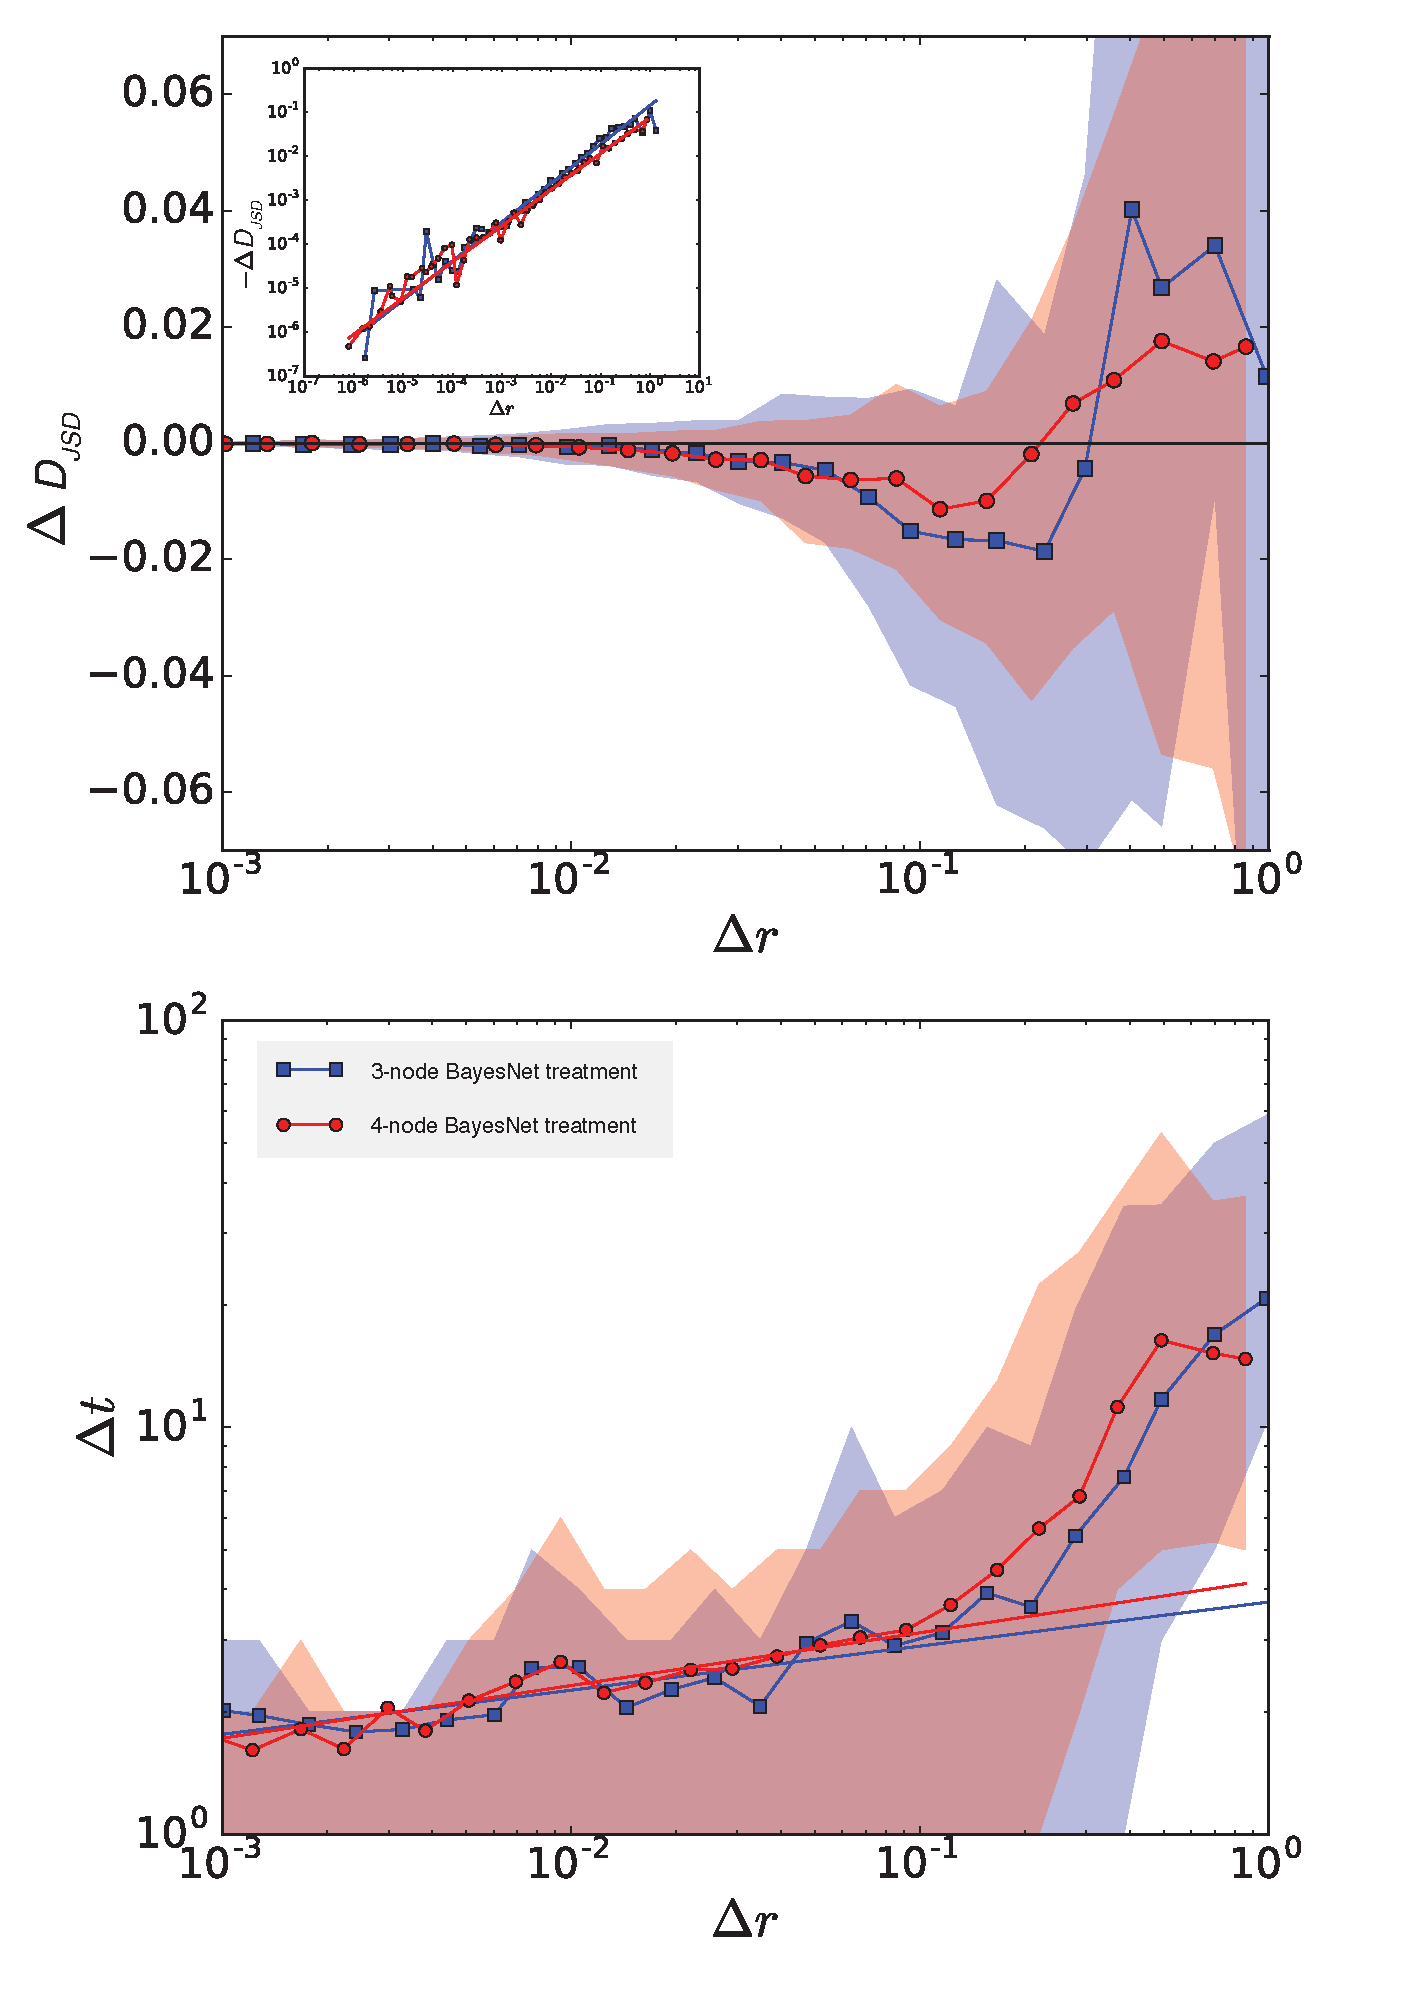
\includegraphics[width=11cm]{figures/vs_dr.pdf}
\caption{{\bf A.} Evolution of the distance to the true model $D$ as a function of displacement $\Delta r$. The distance scales as $D \sim {\Delta r}^{\mu}$ with $\mu_{simple} = 0.88(1)$ [resp. $\mu_{complex} = 082(2)$]. For $\Delta r > 0.2$, $D$ becomes quickly highly uncertain, but rather positive, reflecting the {\it cost} of the making ``wild"displacements. {\bf B} For $\Delta r < 0.2$, the waiting time before a displacement decision is made scales as $\Delta t \sim \Delta r^{\gamma}$ with $\gamma_{simple} = 0.11(1)$ [resp. $\gamma_{complex} = 0.13(1)$]. For $\Delta r > 0.2$, the waiting time before a displacement decision is taken get disproportionally long (up to tens of seconds on average for displacement of 0.7 (i.e., $\approx 25\%$ of the maximum displacement distance). On both panels, blue and red areas show the 25th percentile confidence intervals.}.
%\caption{Scaling relation between $\Delta t$ and $\Delta r$ for the simple (A) and complex (B) treatments. The functions are similar for both treatments [resp. $\sim 0.44(2)$ ($p < 0.01$ , $r = 0.39$) and $\sim 0.47(2)$ ($p < 0.01$ , $r = 0.36$)]. {\bf Actually, one may see this figure differently : scaling $\Delta t \sim {\Delta r}^{0.2}$ for $\Delta r < 0.2$ and another (unknown) regime for $\Delta r > 0.2$ with waiting time getting disproportionately long $\rightarrow$ This may highlight the processing costs associated with a big jump.}}
\label{fig:vs_dr}
\end{center}
\end{figure}


\begin{figure}[h!]
\begin{center}
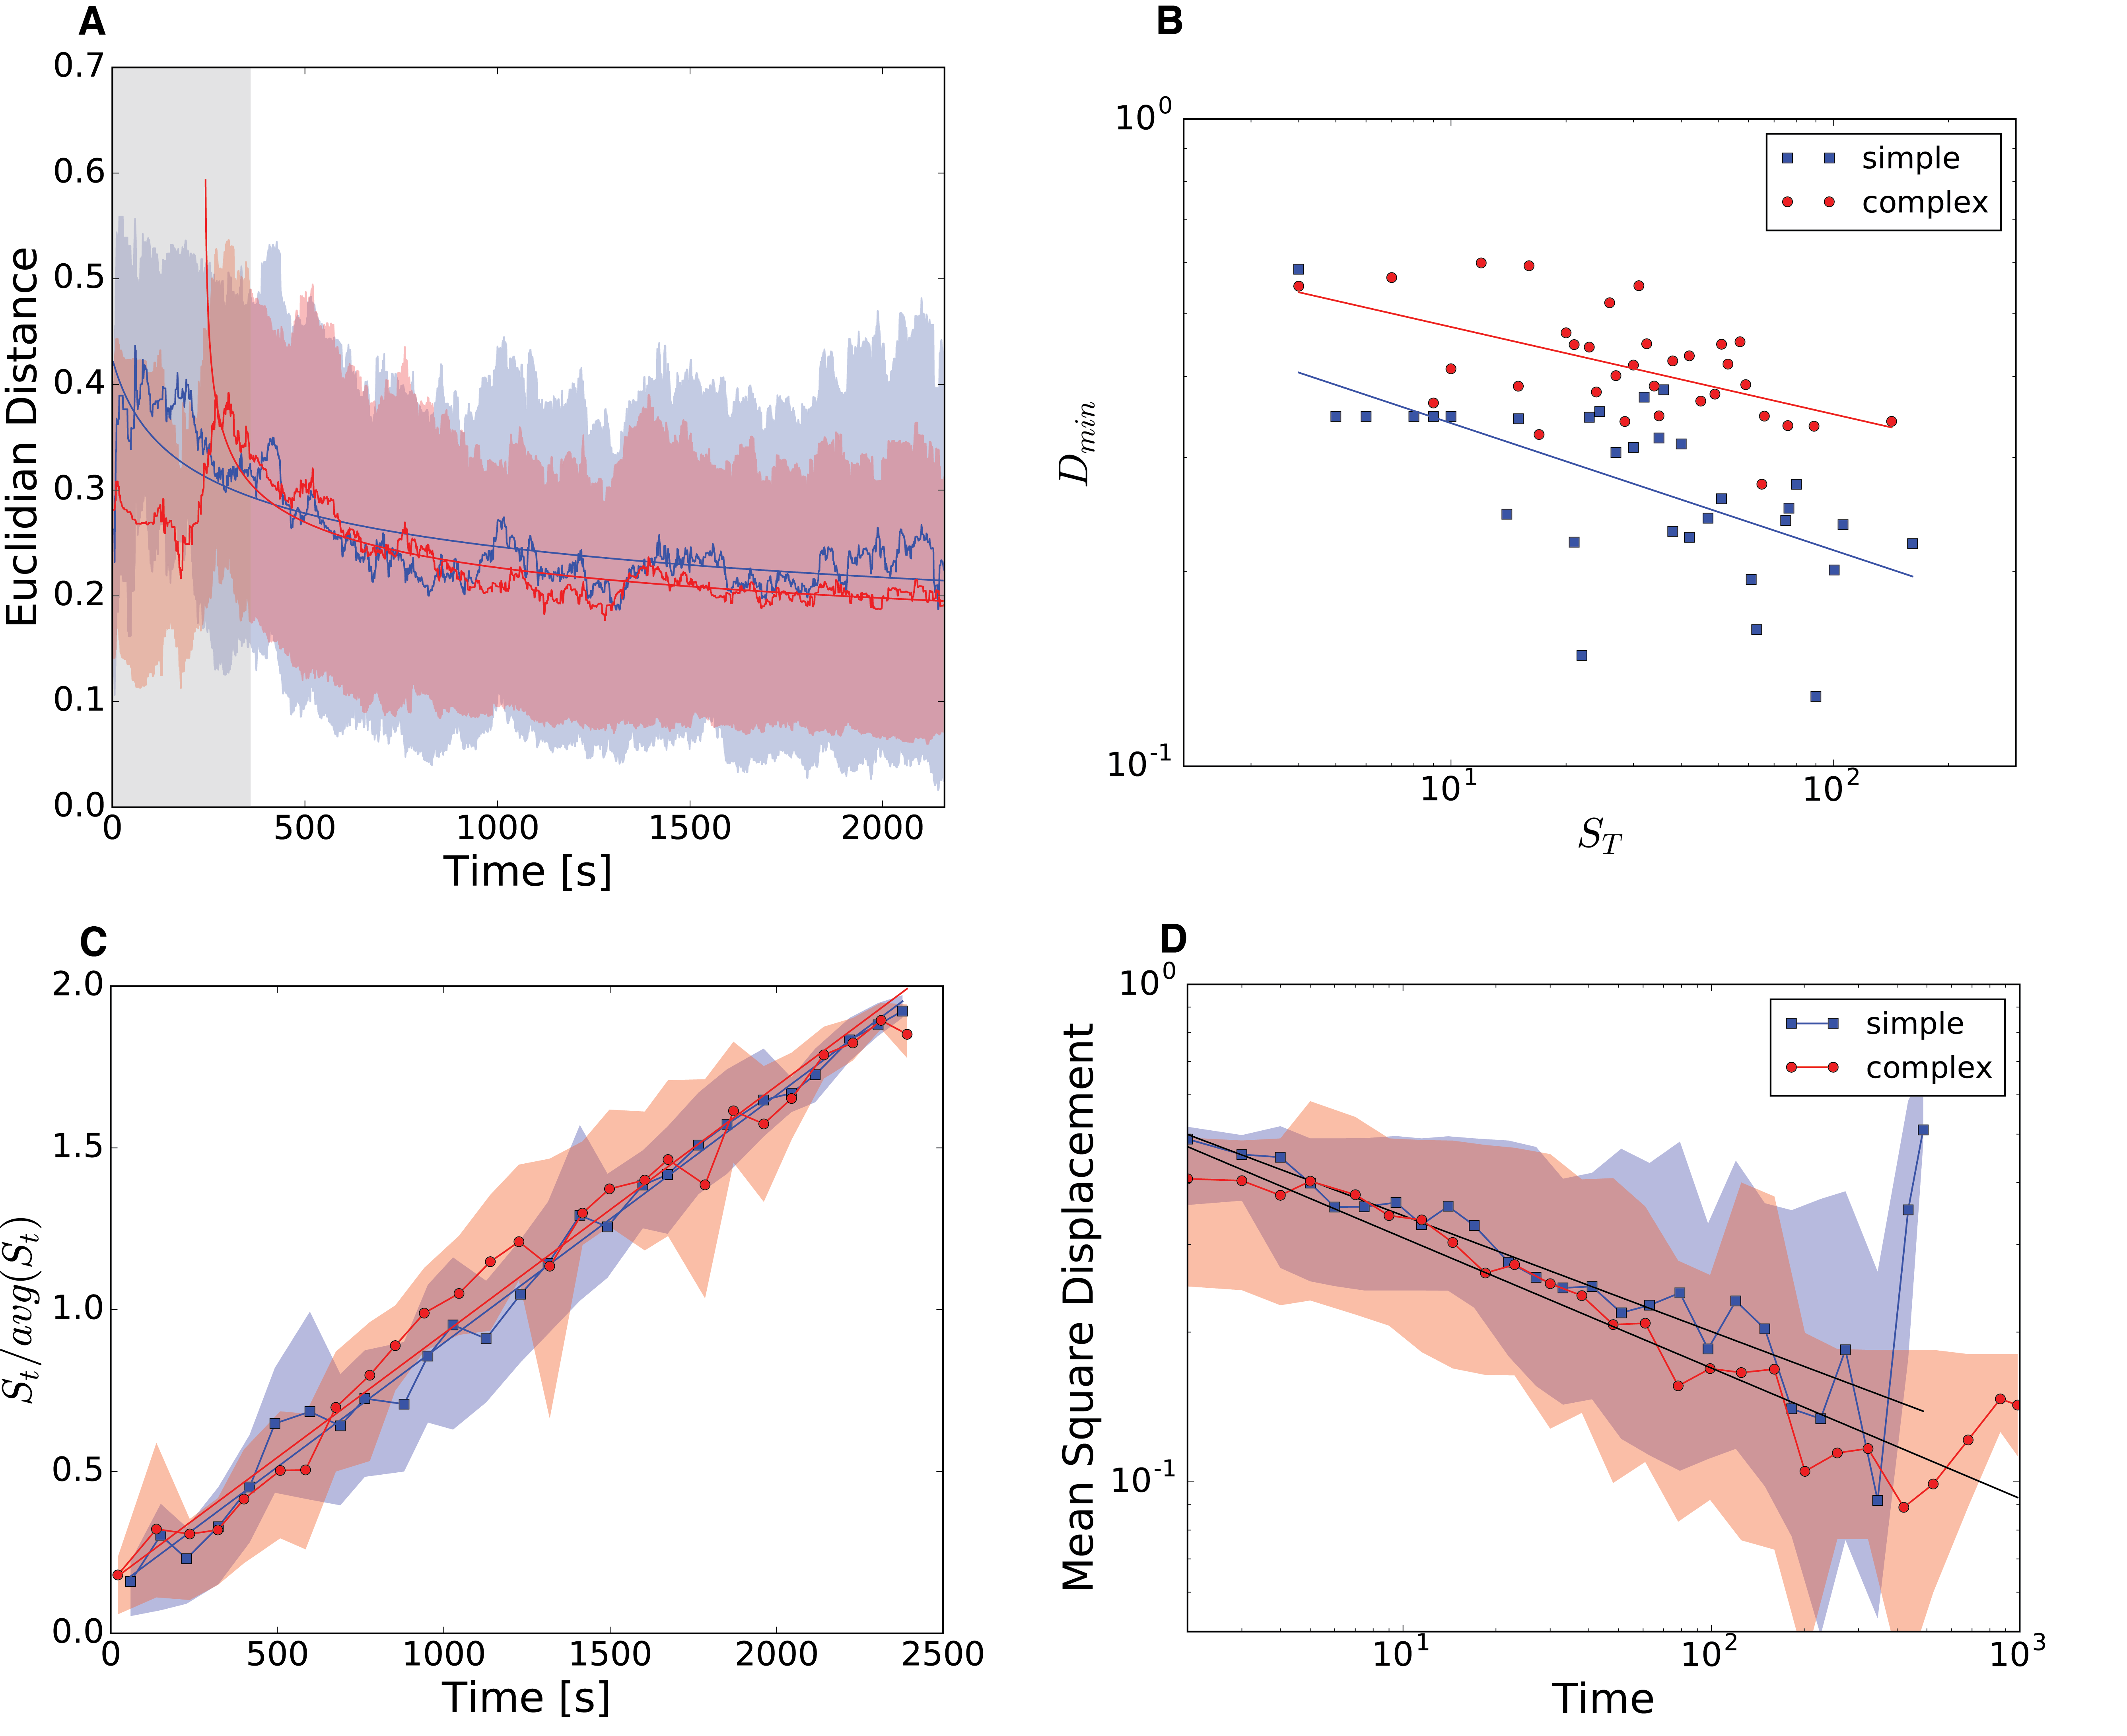
\includegraphics[width=16cm]{figures/Dmin_vs_St.png}
\caption{{\bf A.} Average Euclidian Distance $\langle D \rangle$ decays as function of time as $\sim t^{\nu}$ with $ \nu \approx -0.15(1)$ indicating a very slow convergence to the true model. {\bf B.} Minimum Euclidian distance $D_{min}$ (between the best model and the true model) exhibits a scaling as a function of the number of distinct sites visited $S_{T}$. $D_{min} \sim S_{T}^{\gamma}$ with resp. $\gamma_{simple} = -0.20(4)$ and $\gamma_{complex} = - 0.13(3)$. {\bf C.} The number of visited sites over time $S_t$ is a linear function of time $t$. Hence, the number of distinct visited sites is a predictor of the minimum distance $D_{min}$ achieved. The result also holds for average distance. {\bf D.} Mean square displacement (MSD) decays as $\sim t^{\mu}$ with $\mu_{simple} =-0.23(2)$ and $\mu_{complex} =- 0.26(1)$ showing a slow convergence (on the contrary of a normal L\'evy flight / CTRW, which is characterized by respectively diffusion $\mu_{Levy} = 1$ or super-diffusion $\mu_{CTRW} = \beta$ \cite{21,23}). All colored areas show the 25th percentile confidence intervals.}
\label{fig:Dmin_vs_St}
\end{center}
\end{figure}



\begin{figure}[h!]
\begin{center}
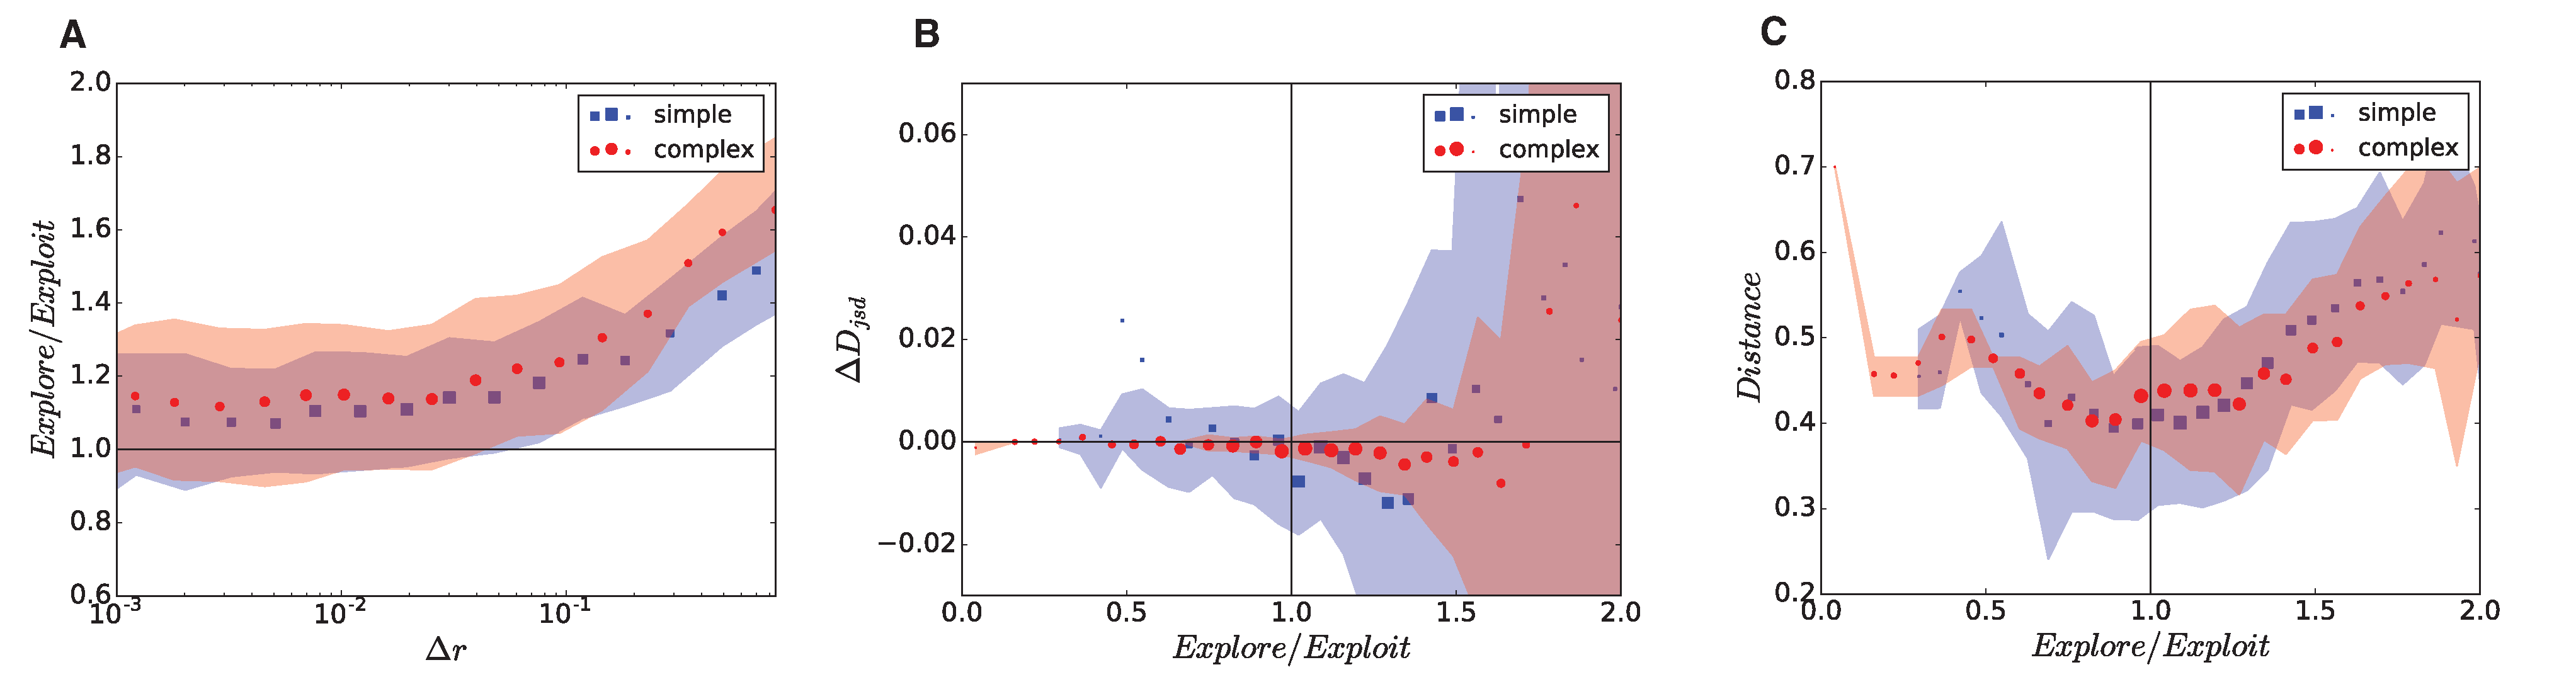
\includegraphics[width=18cm]{figures/EE.eps}
\caption{{\bf A.} Explore / Exploit ($EE$ )as a function of displacement $\Delta r$. {\bf B.} $\Delta D_{jsd}$ as a function Explore / Exploit: Improvement seems better for $EE \approx 1.4$. {\bf C.} $D_{jsd}$ as a function of $EE$: As distance gets smaller, a balance around $EE = 1$ seems to be reached.}
\label{fig:pdf_return}
\end{center}
\end{figure}

\begin{figure}[h!]
\begin{center}
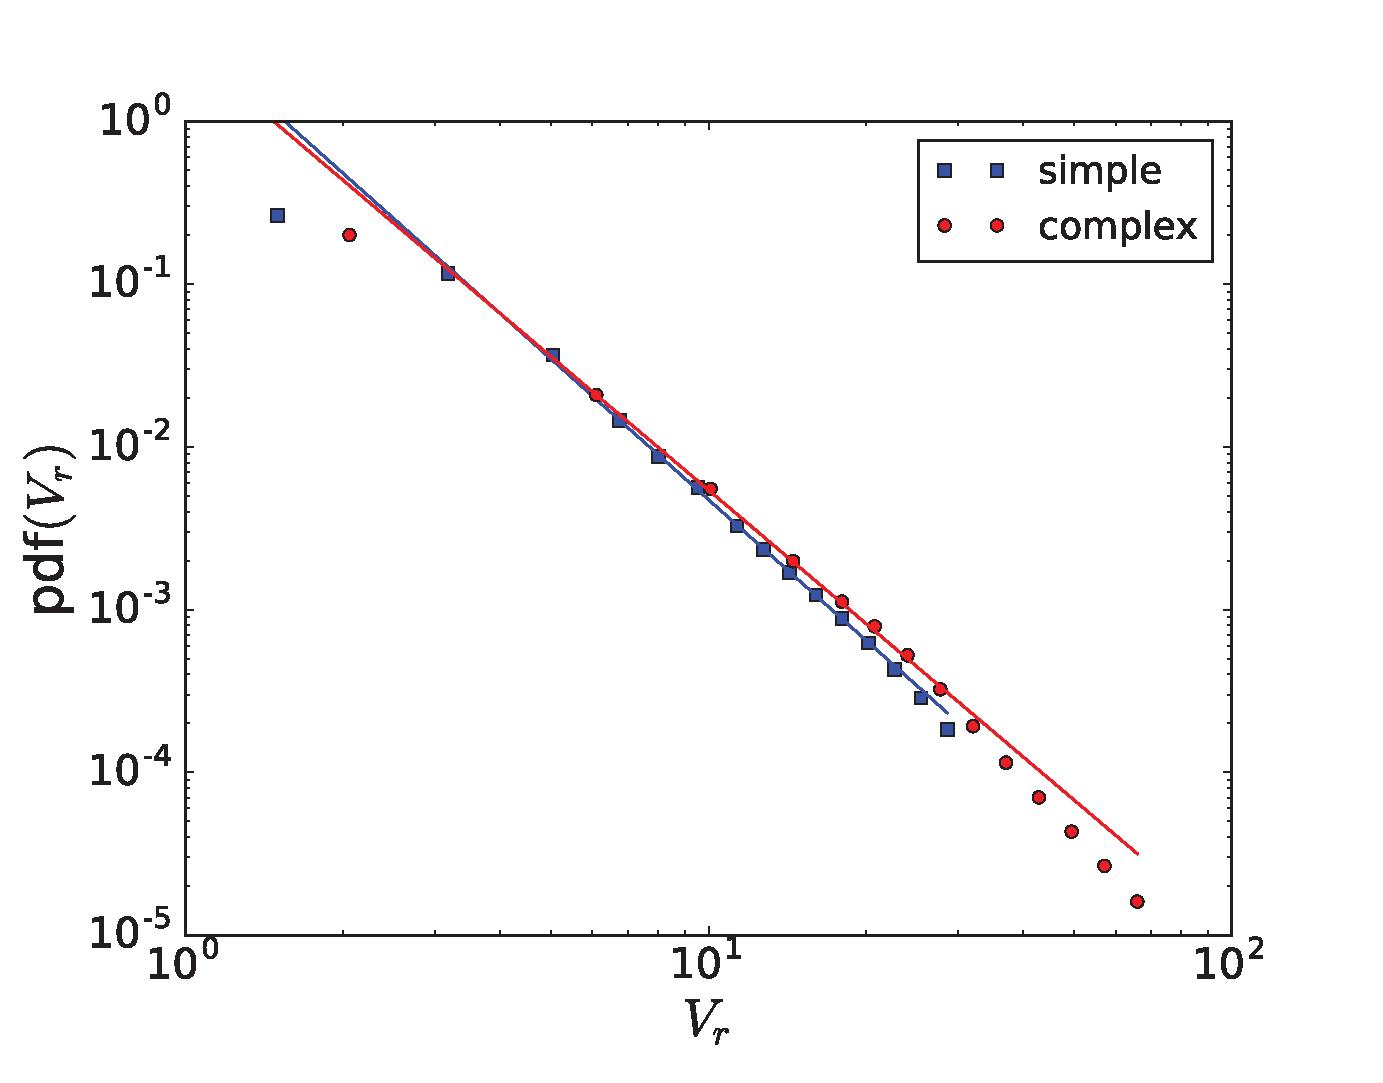
\includegraphics[width=10cm]{figures/pdf_return.eps}
\caption{return to previously visited sites : $\mathrm{pdf}(V_r) \sim {V_r}^{- \gamma -1}$, with $\gamma_{simple} = 1.6(1)$ and $\gamma_{complex} = 1.5(1)$ $\rightarrow$ tendency to return to previously visited sites : This goes against the imperative to visit new sites (maximize $S_T$) in order to reduce $D_{min}$ (c.f. Figures \ref{fig:Dmin_vs_St}B and \ref{fig:Dmin_vs_St}C). Moreover, given the large number of sites [$10^{8}$ (resp. $10^{16}$) in the simple (resp. complex) case], it is remarkable that participants tend to return to exactly the same (tiny) spots. This suggest some stickiness of memory.}
\label{fig:pdf_return}
\end{center}
\end{figure}




\begin{figure}[h!]
\begin{center}
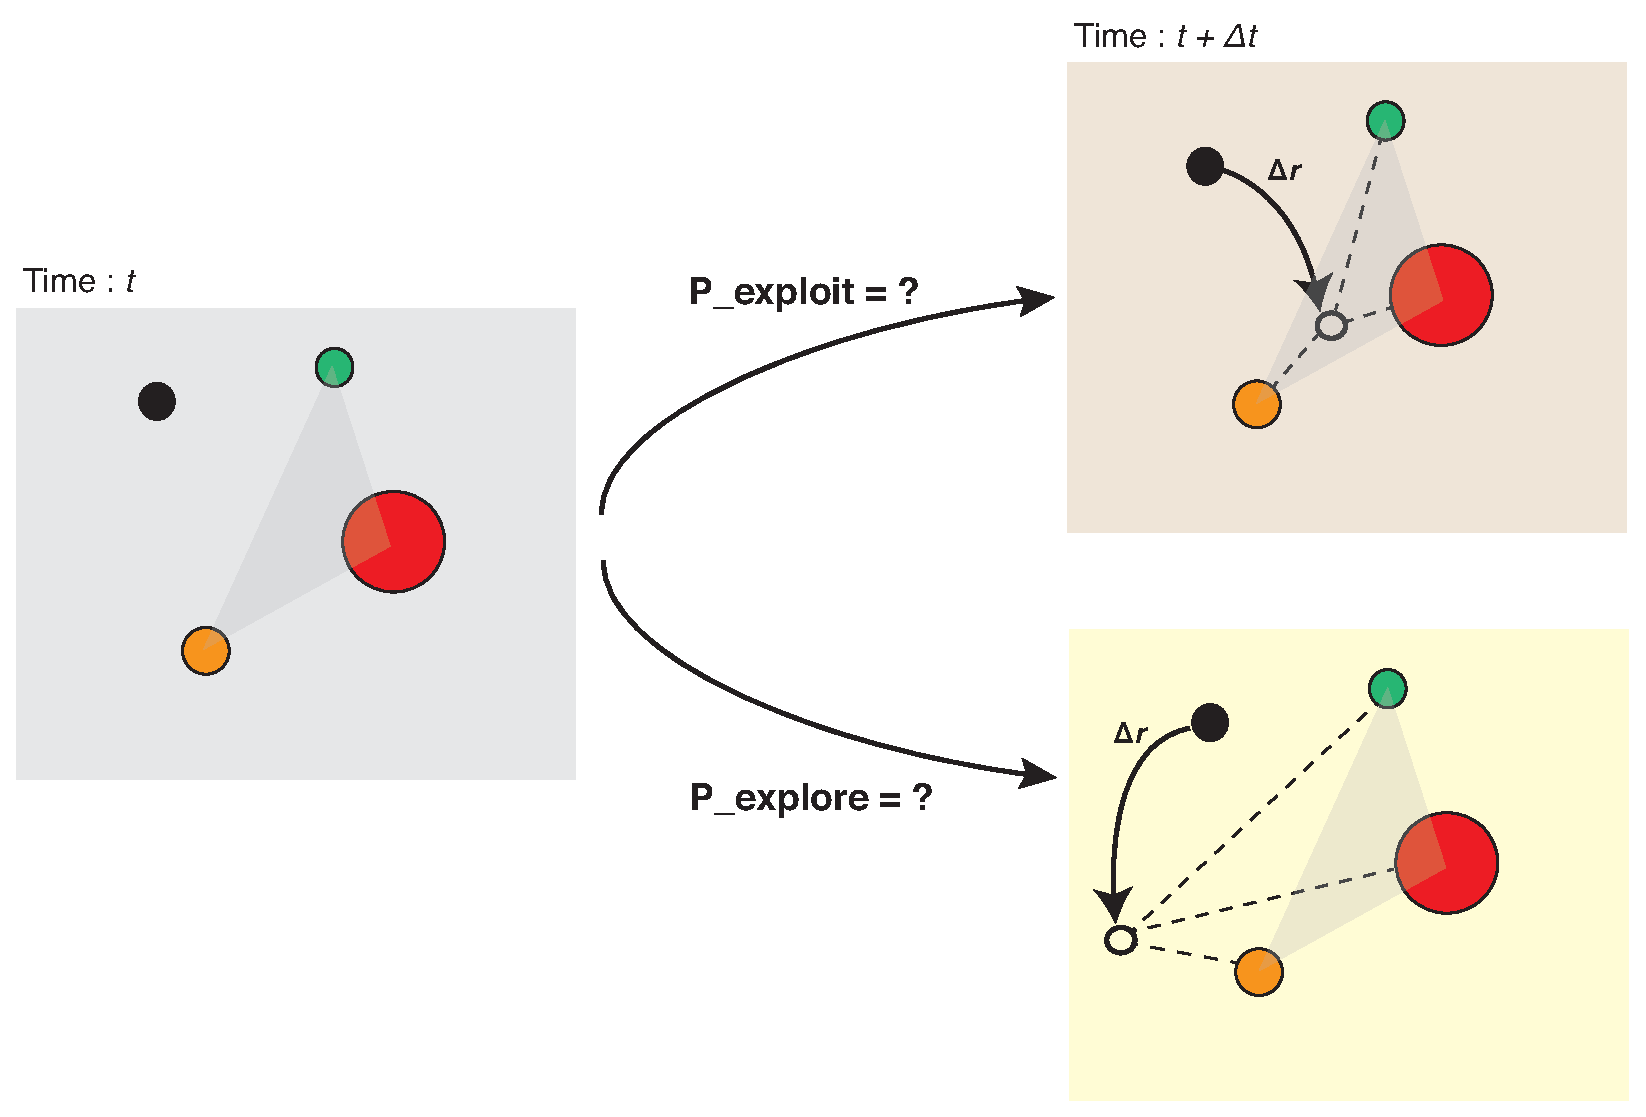
\includegraphics[width=12cm]{figures/schematic_displacement.eps}
\caption{2-dimensional schematic description of the {\it L\'evy flying mind} model ({\bf ``Proportional Attraction"}): At each time step, the individual must choose between remaining in the solution envelope that has already been explored and exploring outside the currently known solution envelope.  We assign some probability $p$ (a number between 0 and 1) to the participant's decision of staying in the explored envelop and probability $1-p$ to the decision to explore outside that envelop.  If it is harder to find solutions that offer a balanced re-combination of previous solutions than to think out-of-the-box and propose solutions outside of the current solution envelope, then $p < \frac{1}{2}$ else $p \geq \frac{1}{2}$.}
\label{fig:schematic}
\end{center}
\end{figure}

%\begin{figure}[h!]
%\begin{center}
%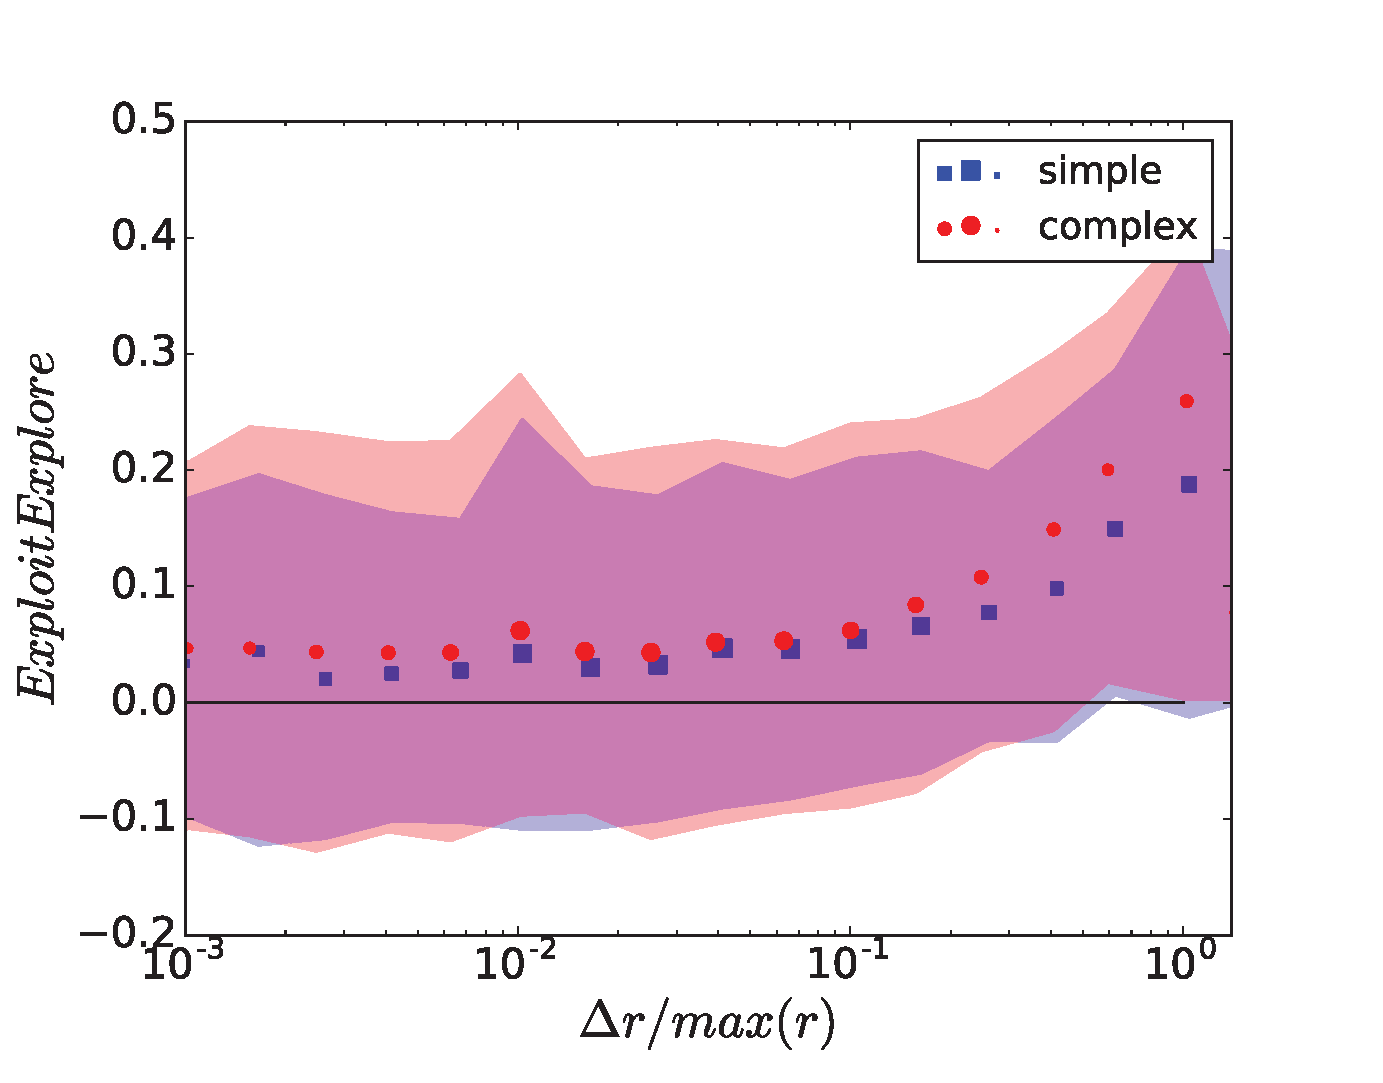
\includegraphics[width=13cm]{figures/EE_vs_Dr.eps}
%\caption{explore exploit}
%\label{fig:exploit_explore}
%\end{center}
%\end{figure}



\begin{figure}[h!]
\begin{center}
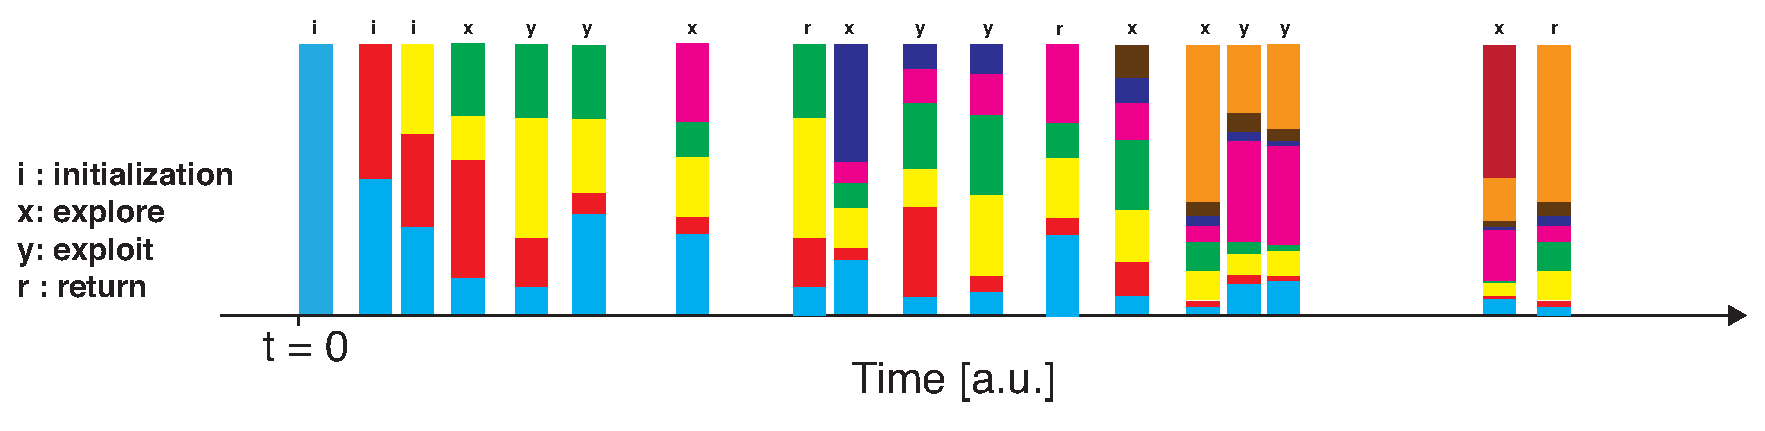
\includegraphics[width=16cm]{figures/schematic_remix.eps}
\caption{Schematic representation of remix dynamics. The color bars show the proportion (i.e., $1/d$) of previously proposed solutions in solution proposed at time $t$. New colors are introduced 	to signal exploration. From time to time, individuals return to previously visited solutions (signaled by $r$).}
\label{fig:schematic_remix}
\end{center}
\end{figure}


\begin{figure}[h!]
\begin{center}
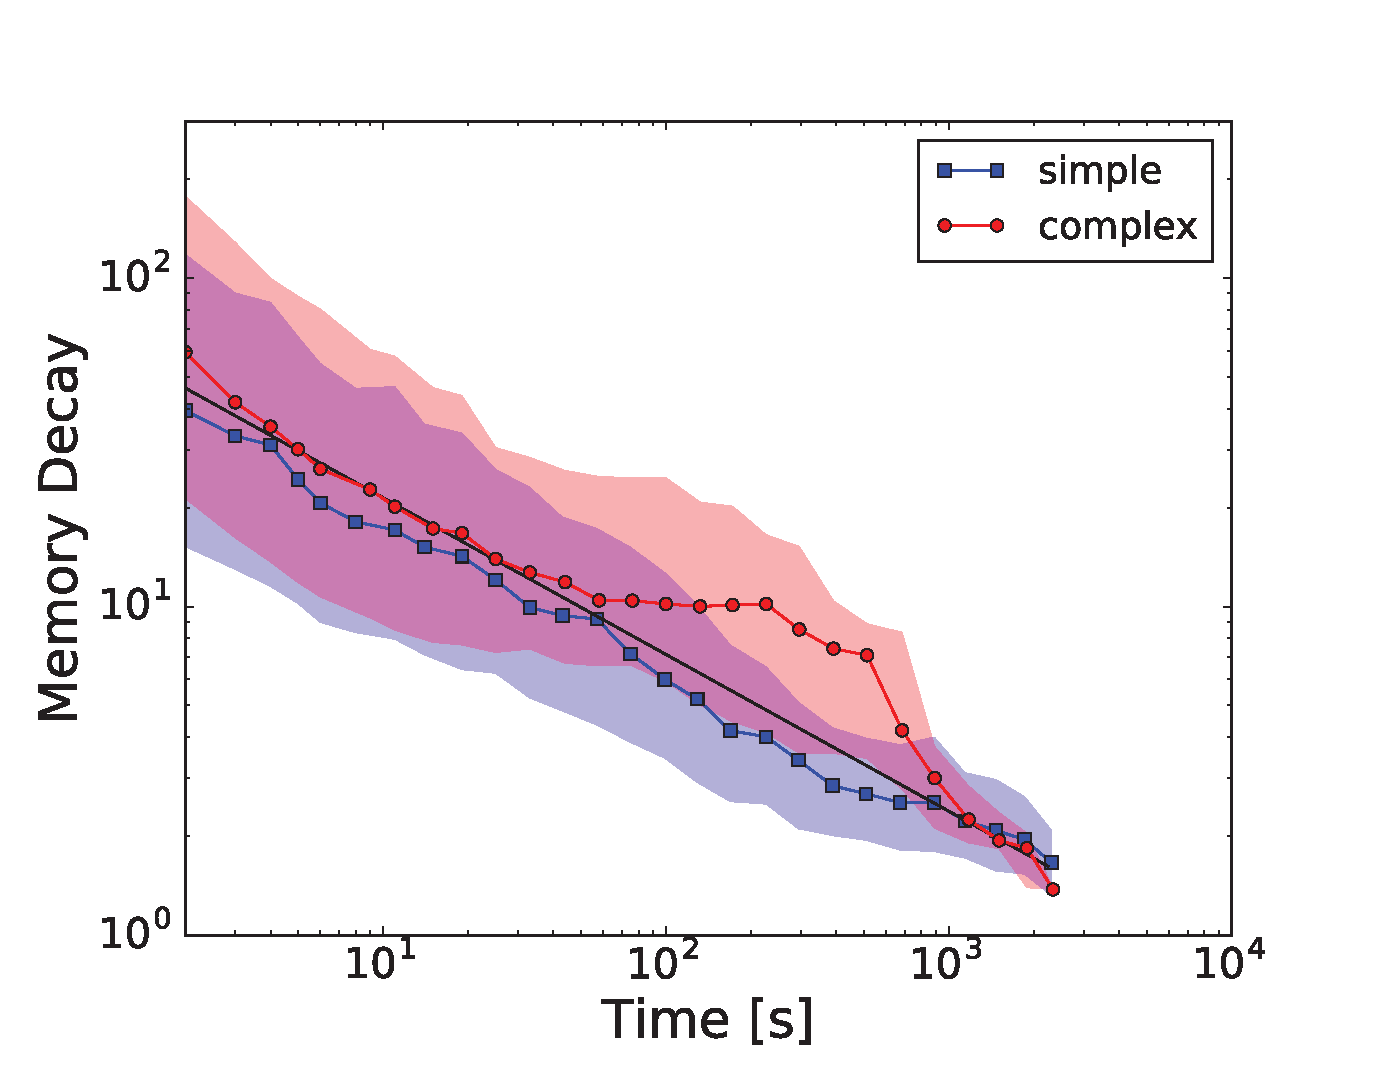
\includegraphics[width=13cm]{figures/MemoryDecay.eps}
\caption{Influence of a model proposed at time in subsequent models. The influence is computed as 1/distance between the focal model and subsequent models. On average over all participants in each treatment, influence $I$ decays as $I \sim t^{-\chi}$ with $\chi = 0.48(2)$ ($p < 0.01$ and $R > 0.32$). This result shows that memory is a long memory process, with implications for the convergence to.}
\label{fig:memory}
\end{center}
\end{figure}



%
%\begin{figure}[h!]
%\begin{center}
%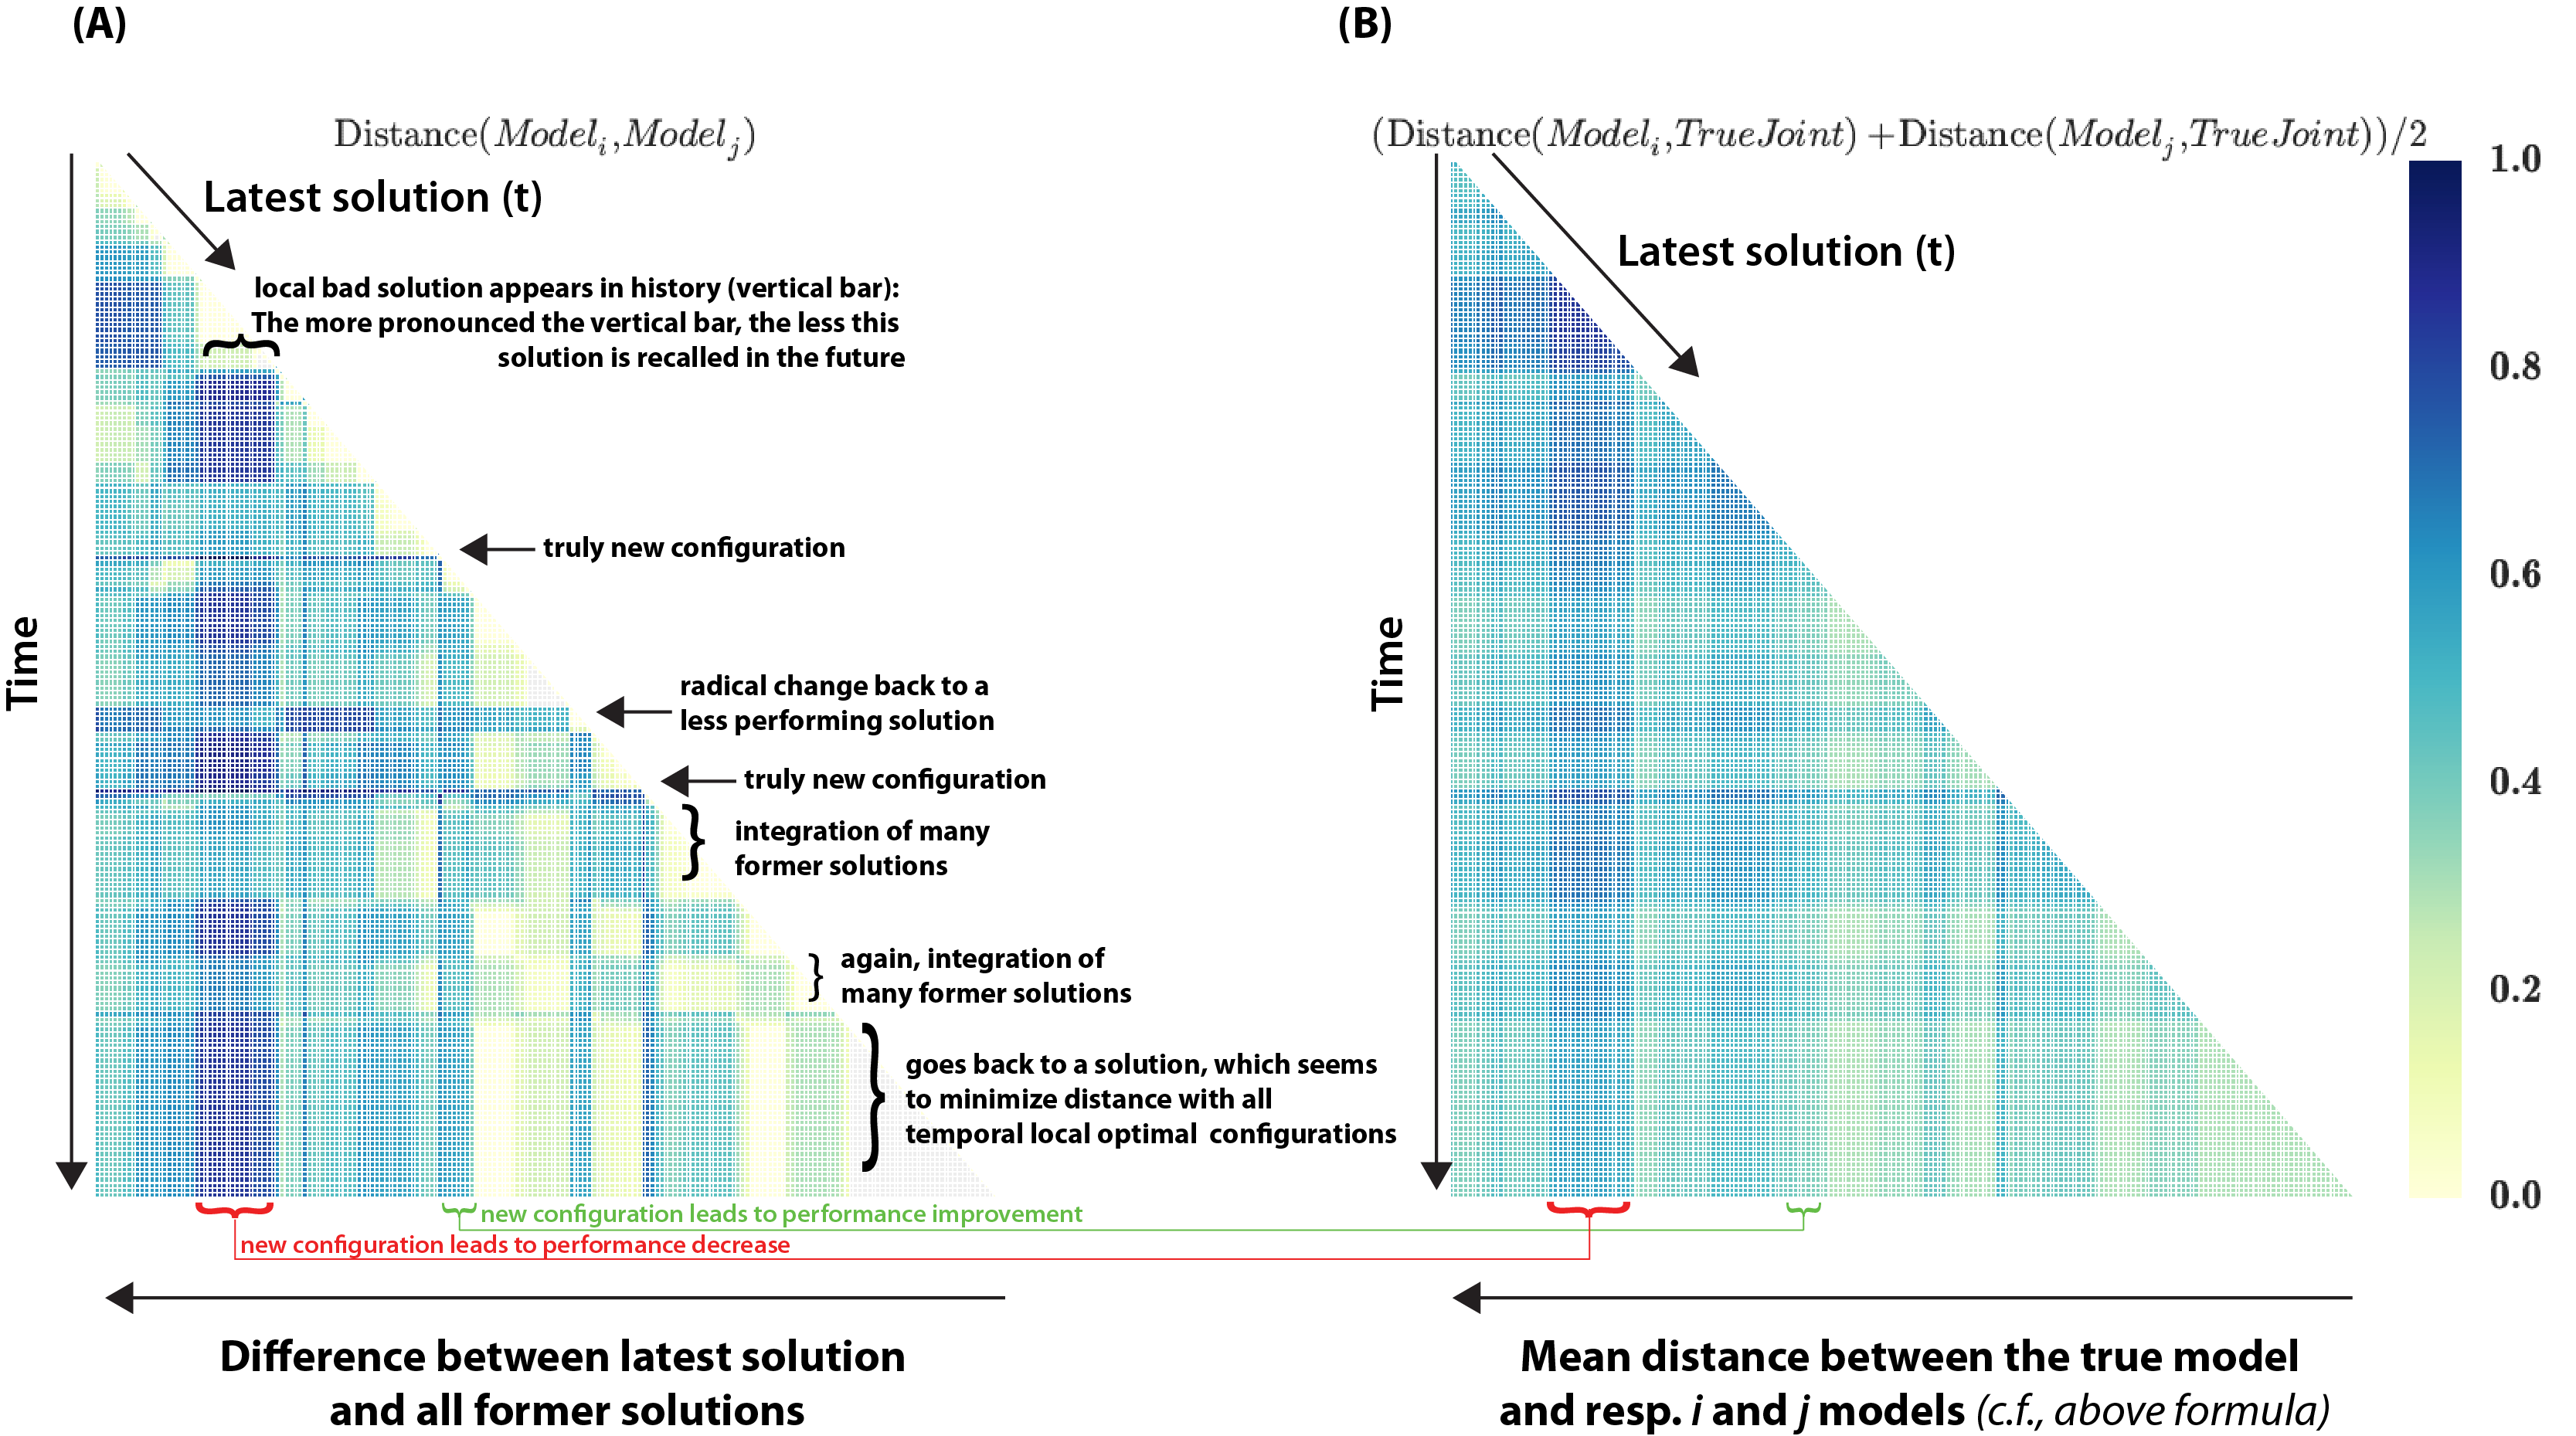
\includegraphics[width=15cm]{figures/matrice2.png}
%\caption{\footnotesize The triangular matrix {\bf A} depicts the cognitive distances between a person's model at time $i$ and that same person's model at time $j$.  latest solution as a function of time and all former solutions, and {\bf B} of mean distance between the true model and resp. $i$ and $j$ configurations. Matrix {\bf B} shows the performance of a proposed model and serves as a reference for rationalizing choice sequences made by participants. These choice sequences are represented in matrix {\bf A} for participant 13: We see a wealth of characteristic choices leading to better of worse solutions, but also some integration and disruptive change in strategies, some which having a positive impact on performance, and other having a negative impact on performance. The rectangle structures show that participants do not drastically update drastically, but rather alternate periods of fine tuning and radical innovation. Matrix {\bf A} can also be watched in a more heuristic way at the coarse grained level: The more contrasted the pattern the more innovation overall. And, as shown here for participant 13, as more models are tested -- towards the lower right corner -- colors get more yellowish showing overall convergence of models. In the case presented here, the convergence of models leads overall to better solutions over time. It may not always be the case.}
%\label{fig:matrices}
%\end{center}
%\end{figure}




